\documentclass[paper=a4, fontsize=11pt]{article}

\usepackage[T1]{fontenc}

\usepackage[utf8]{inputenc}
\usepackage[francais]{babel}
\usepackage{mathtools}
\usepackage{amssymb}
\usepackage{bm}
\usepackage{alltt}
\usepackage{float}
\usepackage{graphicx}
\usepackage[colorinlistoftodos]{todonotes}
\usepackage{geometry}
\usepackage{hyperref}
\usepackage{enumitem}
\usepackage{subcaption}
\usepackage[ruled,vlined]{algorithm2e}

\newcommand{\argmin}[1]{\underset{#1}{\operatorname{argmin}}\;}

\title{\normalfont \normalsize
\huge Pointing error correction}

\author{Jules Kozolinsky, Vincent Matthys}

\date{}

\begin{document}
\maketitle

\section{Attitude of a Satellite}

\begin{figure}[h]
	\centering
	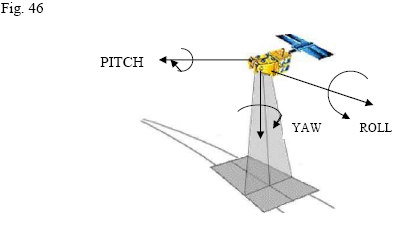
\includegraphics[width=0.5\textwidth]{figures/angles.jpg}
   \caption{ Roll, pitch and yaw angles.}
   \label{angles}
\end{figure}

\section{Satellite attitude error effects on stereo images}
\label{sec:sensibility}

\section{Correction of Relative Pointing Error}
\cite{de2014automatic}\\

A simple way to correct the relative pointing error is thus to transform one of the two images, in such a way that the corresponding points fall on the respective epipolar curves: given two images $u$, $v$ and a set of correspondences $(\textbf{x}_i , \textbf{x}'_i)_{i=1...N}$ , we search for a translation $f$ such that, for all $i$, the transformed point $f(\textbf{x}'_i)$ lies on the epipolar curve $epi^{\textbf{x}_i}_{u v}(R)$.
The desired transformation $f^{*}$ minimises the relative pointing error defined by:
\begin{align}
\label{minif}
f^* = \argmin{f} \dfrac{1}{N} \sum\limits_{i=1}^{N} d(f(\textbf{x}'_i), epi^{\textbf{x}_i}_{u v}(R))
\end{align}

From  \cite{de2014automatic}, we know that the epipolar curve $epi^{\textbf{x}_i}_{u v}(R)$ is approximated up to $0.05$ pixels by the straight line $F\textbf{x}_i$, where $F$ is
the affine fundamental matrix between the two views for the considered tile. As this fundamental matrix is an \textit{affine} fundamental matrix, all the lines $F\textbf{x}_i$ are parallel. Without any additional restriction, we may assume that these lines are horizontal (otherwise just do a change of coordinates). The horizontal line $F\textbf{x}_i$ can be written, in homogeneous coordinates, as
\begin{align*}
F\textbf{x}_i = \left[ 0 \; 1 \; c_i \right]
\end{align*}
With these notations, for each point correspondence $(\textbf{x}_i , \textbf{x}'_i)$, we have
\begin{align*}
e(\textbf{x}_i, \textbf{x}'_i) = d(\textbf{x}'_i, epi^{\textbf{x}_i}_{u v}(R)) = d(\textbf{x}'_i, F\textbf{x}_i) = | y'_i + c_i|
\end{align*}

\subsection{Roll and Pitch Angles}
Because of sensitivity issues, we can take only roll and pitch error into account. Therefore according to section \ref{sec:sensibility}, we search for a transformation $f$ such that
\begin{align*}
f(\textbf{x}) = T\textbf{x}
\end{align*}
where $T$ is a translation.\\
Here the error $e$ is invariant to any horizontal translation, thus the search for a translation minimizing the relative pointing error of formula (\ref{minif}) can be restricted to vertical translations only. With a vertical translation of parameter $t$, the error becomes
\begin{align*}
\dfrac{1}{N} \sum\limits_{i=1}^{N} d(T\textbf{x}'_i, F\textbf{x}_i) = \dfrac{1}{N} \sum\limits_{i=1}^{N} | y'_i + t+ c_i|
\end{align*}
The translation that minimizes this sum is given by the geometric median (Weiszfeld, 1937) of the vector $(-y'_i - c_i )_{i=1...N}$.  The relative pointing error can thus be minimized in a tile by applying a translation to one of the images. Note that the median is robust against outliers, thus this correction procedure works well even in the presence of false matches.

\subsection{Roll, Pitch and Yaw Angles}
If we assume that the scene is located at infinity with respect to the satellite, an error in the sensor attitude measurement can be modeled in image space as a translation composed with a rotation. Therefore we have
\begin{align*}
f(\textbf{x}) = RT\textbf{x}
\end{align*}
where $R$ is a rotation and $T$ a translation.\\

\appendix

Reminder: Matrix multiplication have always the origin as a fixed point. Common workaround using homogeneous coordinates.

\section{Rotations and translation}

In this part, we consider any point \((x, y) \in \mathbb{R}^2\). As translation and rotation do not commute, we will consider two cases: rotation followed by translation and translation followed by rotation, with \(R\) denoting the rotation of angle \(\theta\) and \(T\) denoting the translation of vector \((t_x, t_y)\). Naming \(f\) the resulting function.

\begin{align*}
	T &=
		\begin{pmatrix}
			1 & 0 & t_x \\
			0 & 1 & t_y \\
			0 & 0 & 1
		\end{pmatrix}
		\\
	R &=
		\begin{pmatrix}
			\cos \theta & -\sin \theta & 0 \\
			\sin \theta & \cos \theta & 0 \\
			0 & 0 & 1
		\end{pmatrix}
\end{align*}


\subsection{Rotation followed by a translation}
This happens when correcting the pointing error first with the rotation.

\begin{align*}
	f(\bm{x}) &= TR\bm{x} \\
	&=
		\begin{pmatrix}
			1 & 0 & t_x \\
			0 & 1 & t_y \\
			0 & 0 & 1
		\end{pmatrix}
		\cdot
		\begin{pmatrix}
			\cos \theta x - \sin \theta y \\
			\sin \theta x + \cos \theta y \\
			1
		\end{pmatrix}
		\\
	&=
		\begin{pmatrix}
			\cos \theta x - \sin \theta y + t_x\\
			\sin \theta x + \cos \theta y + t_y\\
			1
		\end{pmatrix}
\end{align*}

\subsection{Translation followed by a rotation}
This happens when correcting the pointing error first with the translation

\begin{align*}
	f(\bm{x}) &= RT\bm{x} \\
	&=
		\begin{pmatrix}
			\cos \theta & -\sin \theta & 0 \\
			\sin \theta & \cos \theta & 0 \\
			0 & 0 & 1
		\end{pmatrix}
		\cdot
		\begin{pmatrix}
			x + t_x \\
			y + t_y \\
			1
		\end{pmatrix} \\
	&=
		\begin{pmatrix}
			\cos \theta (x + t_x) - \sin \theta (y + t_y)\\
			\sin \theta (x + t_x) + \cos \theta (y + t_y)\\
			1
		\end{pmatrix}
\end{align*}


\bibliographystyle{plain}
\bibliography{biblio}
\end{document}
